\documentclass{beamer}
\usetheme{metropolis}
\usepackage{graphicx}
\usepackage{subfig}
\usepackage{tcolorbox}
\title{A History of Science in Latin America (INTD262): Unit 0}
\author{Jordan Hanson}
\institute{Whittier College Department of Physics and Astronomy}

\begin{document}
\maketitle

\section{Summary}

\begin{frame}{Unit 0 Summary}
\footnotesize
\textbf{The Scientific Attitude, Nomenclature, Mesoamerican Science}
\begin{enumerate}
\item The Demarcation Problem: the line between science and non-science
\item Nomenclature: philosophical, ecclesiastical, geographical, and political
\item \textit{Reading and discussion}
\begin{itemize}
\footnotesize
\item \alert{The Introduction and Chapter 1 of \textit{The Scientific Attitude}}
\begin{enumerate}
\item Examples of good science in 19th century medicine
\item Examples of denialism, pseudo-science, and fraud
\end{enumerate}
\item \alert{Introduction and Chapter 1 of \textit{Science in Latin America}}
\begin{enumerate}
\item Examples of botany, zoology, and medicine of indigenous 18th-century Mexican people
\item Comparisons to colonial knowledge and medieval medicine
\item Examples of knowledge transmission: Europe to Latin America, and Latin America to Europe
\end{enumerate}
\end{itemize}
\end{enumerate}
\end{frame}

\begin{frame}{Unit 0 In-class activities}
\small
\textit{In-class group activities}
\begin{itemize}
\small
\item The Mayan numeric system, comparitive mathematics
\item Classification of studies: science or non-science?
\item Classification of species: hummingbirds
\item Medicine: malaria and its treatmeant with quinine
\end{itemize}
\begin{figure}
\centering
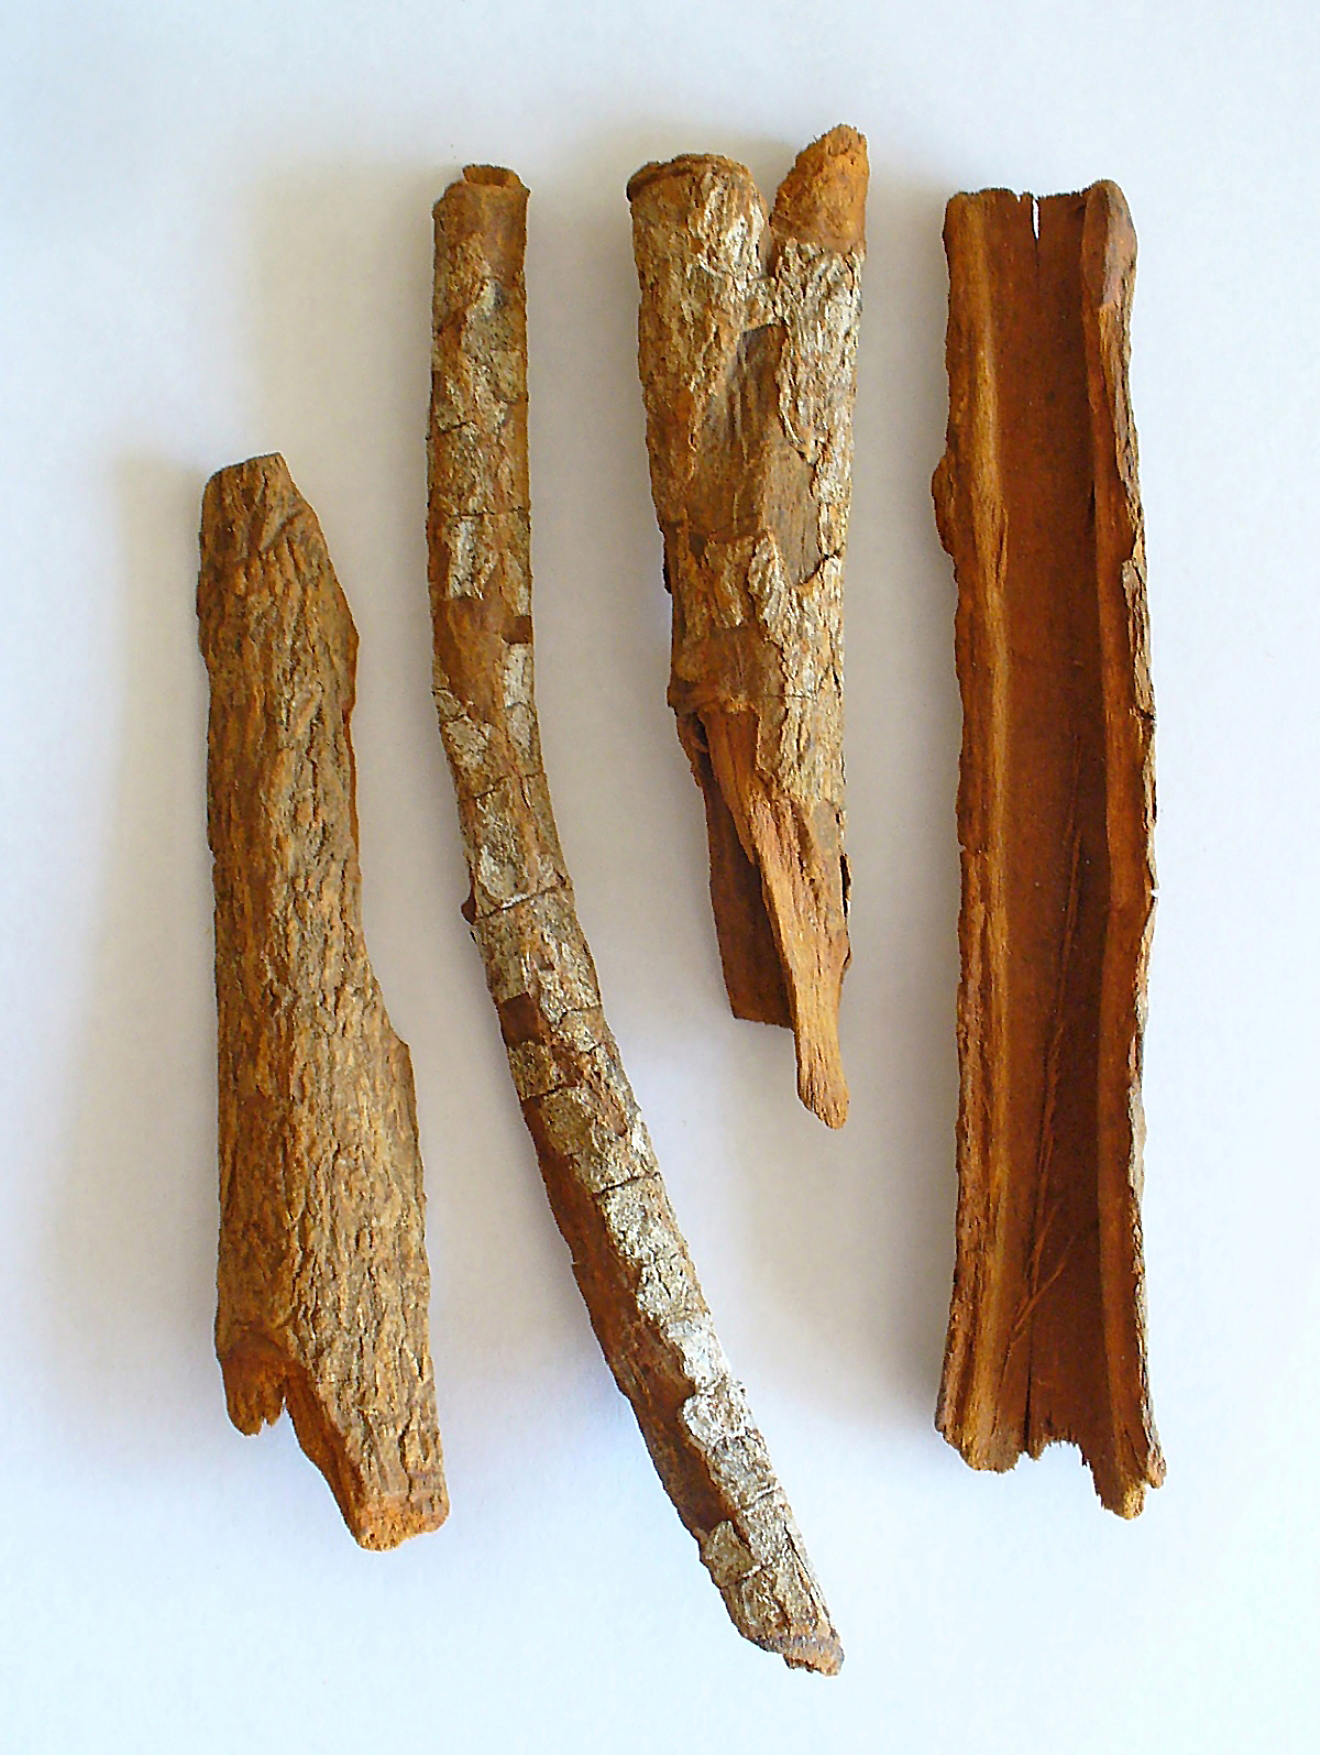
\includegraphics[width=0.2\textwidth]{figures/cinchona.jpeg}
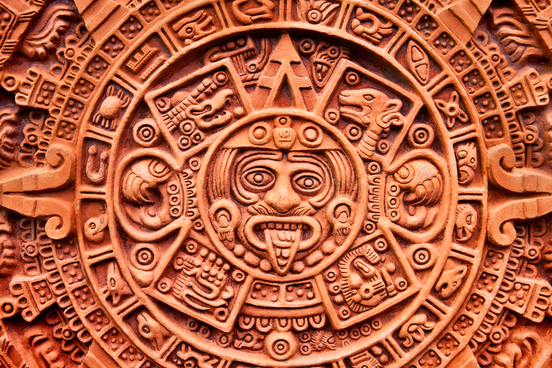
\includegraphics[width=0.4\textwidth]{figures/aztec.jpg}
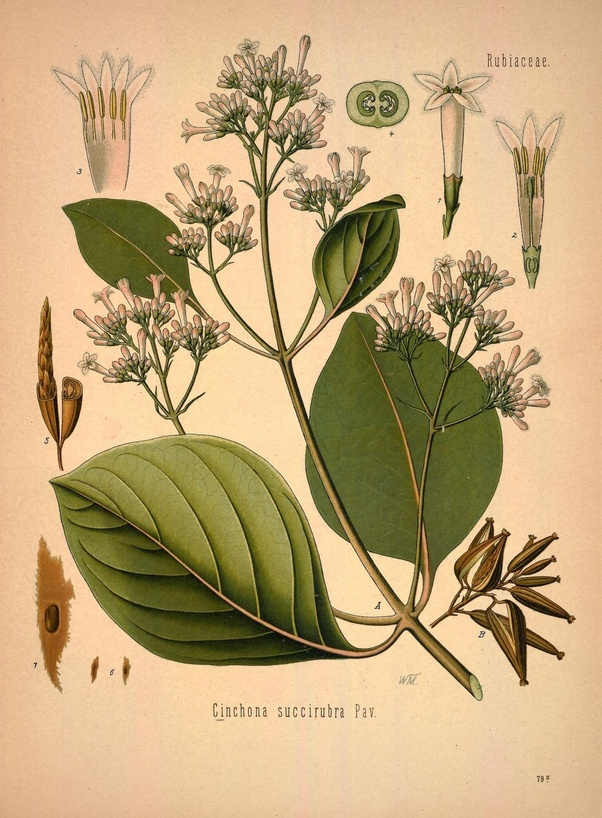
\includegraphics[width=0.195\textwidth]{figures/cinchona2.jpeg}
\end{figure}
\end{frame}

\begin{frame}{Course Texts}
\begin{figure}
\centering
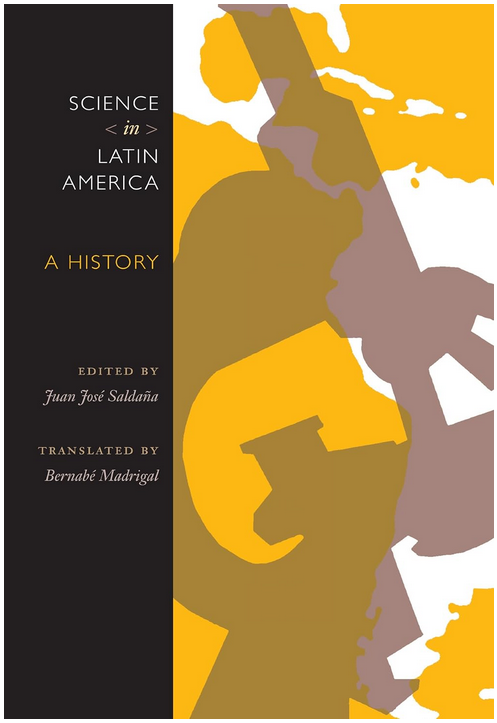
\includegraphics[width=0.4\textwidth]{figures/book1.png}

\includegraphics[width=0.4\textwidth]{figures/book2.png}
\caption{\label{fig:1} (Left) \textit{Science in Latin America: A History}, edited by Salda\~{n}a. (Right) \textit{The Scientific Attitude}, by Lee McIntyre.}
\end{figure}
\end{frame}

\section{The Demarcation Problem: the line between science and non-science}

\begin{frame}{The Demarcation Problem: the line}
\textit{If we are asked to determine whether a human activity is scientific, what criteria should we use?} \\ \vspace{0.5cm}
\begin{columns}[T]
\begin{column}{0.5\textwidth}
\textbf{Non-scientific activities:}
\begin{enumerate}
\item 
\item 
\item 
\item 
\item 
\end{enumerate}
\end{column}
\begin{column}{0.5\textwidth}
\textbf{Scientific activities:}
\begin{enumerate}
\item 
\item 
\item 
\item 
\item 
\end{enumerate}
\end{column}
\end{columns} \vspace{0.5cm}
Can we derive any \textbf{\alert{specific criteria}} that distinguish the lists?
\end{frame}

\begin{frame}{The Demarcation Problem: the scientific method}
\textit{How do we define \textbf{the scientific method}?  Let's re-create the scientific method for (left column) the physical sciences, (middle column) the life sciences, and (right column) the social sciences.} \\ \vspace{0.5cm}
\begin{columns}[T]
\begin{column}{0.33\textwidth}
\textbf{Physical Sciences:}
\begin{enumerate}
\item 
\item 
\item 
\item 
\item 
\end{enumerate}
\end{column}
\begin{column}{0.33\textwidth}
\textbf{Life Sciences:}
\begin{enumerate}
\item 
\item 
\item 
\item 
\item 
\end{enumerate}
\end{column}
\begin{column}{0.33\textwidth}
\textbf{Social Sciences:}
\begin{enumerate}
\item 
\item 
\item 
\item 
\item 
\end{enumerate}
\end{column}
\end{columns}
\end{frame}

\begin{frame}{The Demarcation Problem: the scientific method}
\small
\textit{Philosophers of science} provide rational justification for scientific results, even while scientific progress continues. \\ \vspace{0.5cm}
\begin{figure}
\centering
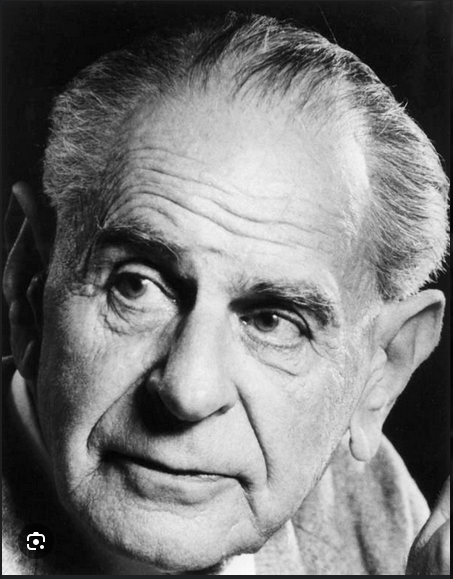
\includegraphics[width=0.385\textwidth]{figures/popper.png}
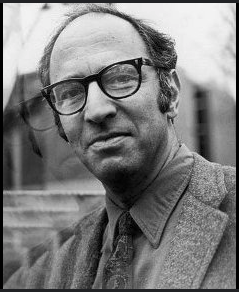
\includegraphics[width=0.4\textwidth]{figures/kuhn.png}
\caption{\label{fig:phil} (Left) Karl Popper, a philosopher of science (1902 - 1994). (Right) Thomas Kuhn, also a philosopher of science (1922 - 1996).}
\end{figure}
\end{frame}

\begin{frame}{The Demarcation Problem: induction and deduction}
\small
\begin{columns}[T]
\begin{column}{0.45\textwidth}
\textbf{Examples of induction:}
\begin{enumerate}
\item ``When I observe hummingbirds, I note they are all green.  Therefore, all hummingbirds are green.''
\item \vspace{0.5cm}
\item \vspace{0.5cm}
\end{enumerate}
\end{column}
\begin{column}{0.45\textwidth}
\textbf{Examples of deduction:}
\begin{enumerate}
\item ``Given that there are no camels in Germany, and that Hamburg is a city in Germany, I know that there are no camels in Hamburg.''
\item \vspace{0.5cm}
\item \vspace{0.5cm}
\end{enumerate}
\end{column}
\end{columns}
\end{frame}

\begin{frame}{The Demarcation Problem: falsification}
\small
\begin{columns}[T]
\begin{column}{0.45\textwidth}
\textbf{Falsifiable scientific hypotheses:}
\begin{enumerate}
\item ``Noble gases are made of molecules, and this leads to a predictable relationship between their temperature, pressure, and volume.''
\item \vspace{0.5cm}
\item \vspace{0.5cm}
\end{enumerate}
\end{column}
\begin{column}{0.45\textwidth}
\textbf{Un-falsifiable scientific hypotheses:}
\begin{enumerate}
\item ``Cutting taxes leads to an increase in economic opportunity for our citizens.''
\item \vspace{0.5cm}
\item \vspace{0.5cm}
\end{enumerate}
\end{column}
\end{columns}
\end{frame}

\begin{frame}{The Demarcation Problem: falsification}
\small
\begin{figure}
\centering
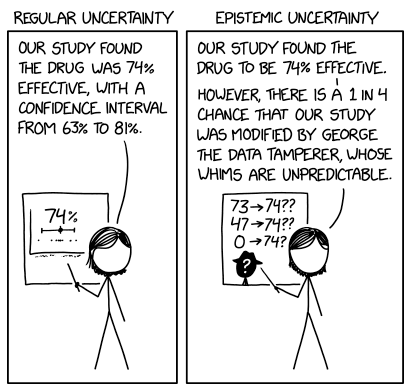
\includegraphics[width=0.6\textwidth]{figures/george.png}
\caption{\label{fig:george} Credit: \url{xkcd.com}.}
\end{figure}
\end{frame}

\section{Nomenclature: philosophical, ecclesiastical, geographical, and political}

\begin{frame}{Nomenclature: philosophical}
\small
\begin{itemize}
\item \textbf{Epistemology}: the philosophy of how we know something to be true
\item \textbf{Metaphysics}: first principles, including abstract concepts such as being, knowing, substance, cause, identity, time, and space.
\item \textbf{Cartesianism}: philosophy of Ren\'{e} Descartes, \textit{Discourse on the Method}, \textit{Geometry}
\begin{itemize}
\footnotesize
\item ``I think, therefore I am.'' Start with doubt, then find concrete ideas in which to place belief
\item \textit{Geometry} was an appendix to \textit{Discourse}, unified algebra and geometry. Translating geometric areas and volumes into algebraic equations was unique and new at the time. From this moment we get the notion of a coordinate system
\item Offered three proofs of the existence of the Lord
\item Also worked on cosmology, optics, and the psychology of emotions
\end{itemize}
\end{itemize}
\end{frame}

\begin{frame}{Nomenclature: philosophical}
\small
\begin{itemize}
\item \textbf{Rationalism}: the theory that reason rather than experience is the foundation of certainty in knowledge
\item \textbf{Empiricism}: the theory that all knowledge is derived from sensory experience, stimulated by the rise of experimental science
\item \textbf{Theology}: the study of the nature of God and religious belief, systematically developed
\begin{itemize}
\item Example of a theologian: Saint Thomas Aquinas (Dominican priest within the Catholic Church, from Sicily).
\begin{itemize}
\item Scholasticism, \textit{Summa Theologica}, reconciling faith and reason, 
\item Influential philosopher from the Medeival period
\item Epistemology, ethics, economics, social justice
\end{itemize}
\end{itemize}
\end{itemize}
\end{frame}

\begin{frame}{Nomenclature: philosphical}
\textbf{Empiricism}: epistemology based on sensory experience
\begin{enumerate}
\item Clearly has implications for experimental science
\item Modern sciences (especially the physical sciences) are divided into three branches:
\begin{itemize}
\item theoretical
\item experimental
\item computational
\end{itemize}
\item Mathematics is also divided into various branches, including applied math, pure mathematics, which itself is divided into topology, algebra, real/complex analysis ...
\end{enumerate}
\end{frame}

\begin{frame}{Nomenclature: ecclesiastical}
\textbf{The Catholic Church}: the Christian Church founded by Jesus of Nazareth.  Adopted the hierarchy of the classical Roman Empire:
\begin{enumerate}
\item Pope - the formal leader of the Church
\item Cardinal, archbishop, bishop, priest
\item Archdiocese, Diocese
\item Orders: Franciscan, Dominican, Society of Jesus (Jesuits)
\item Monks, nuns, priests from orders, and from dioceses
\end{enumerate}
\textbf{Role in teaching}: often in the colonial period, modern universities grew from universities founded and run by the Catholic Church
\end{frame}

\begin{frame}{Nomenclature: geographic and political}
\begin{figure}
\centering
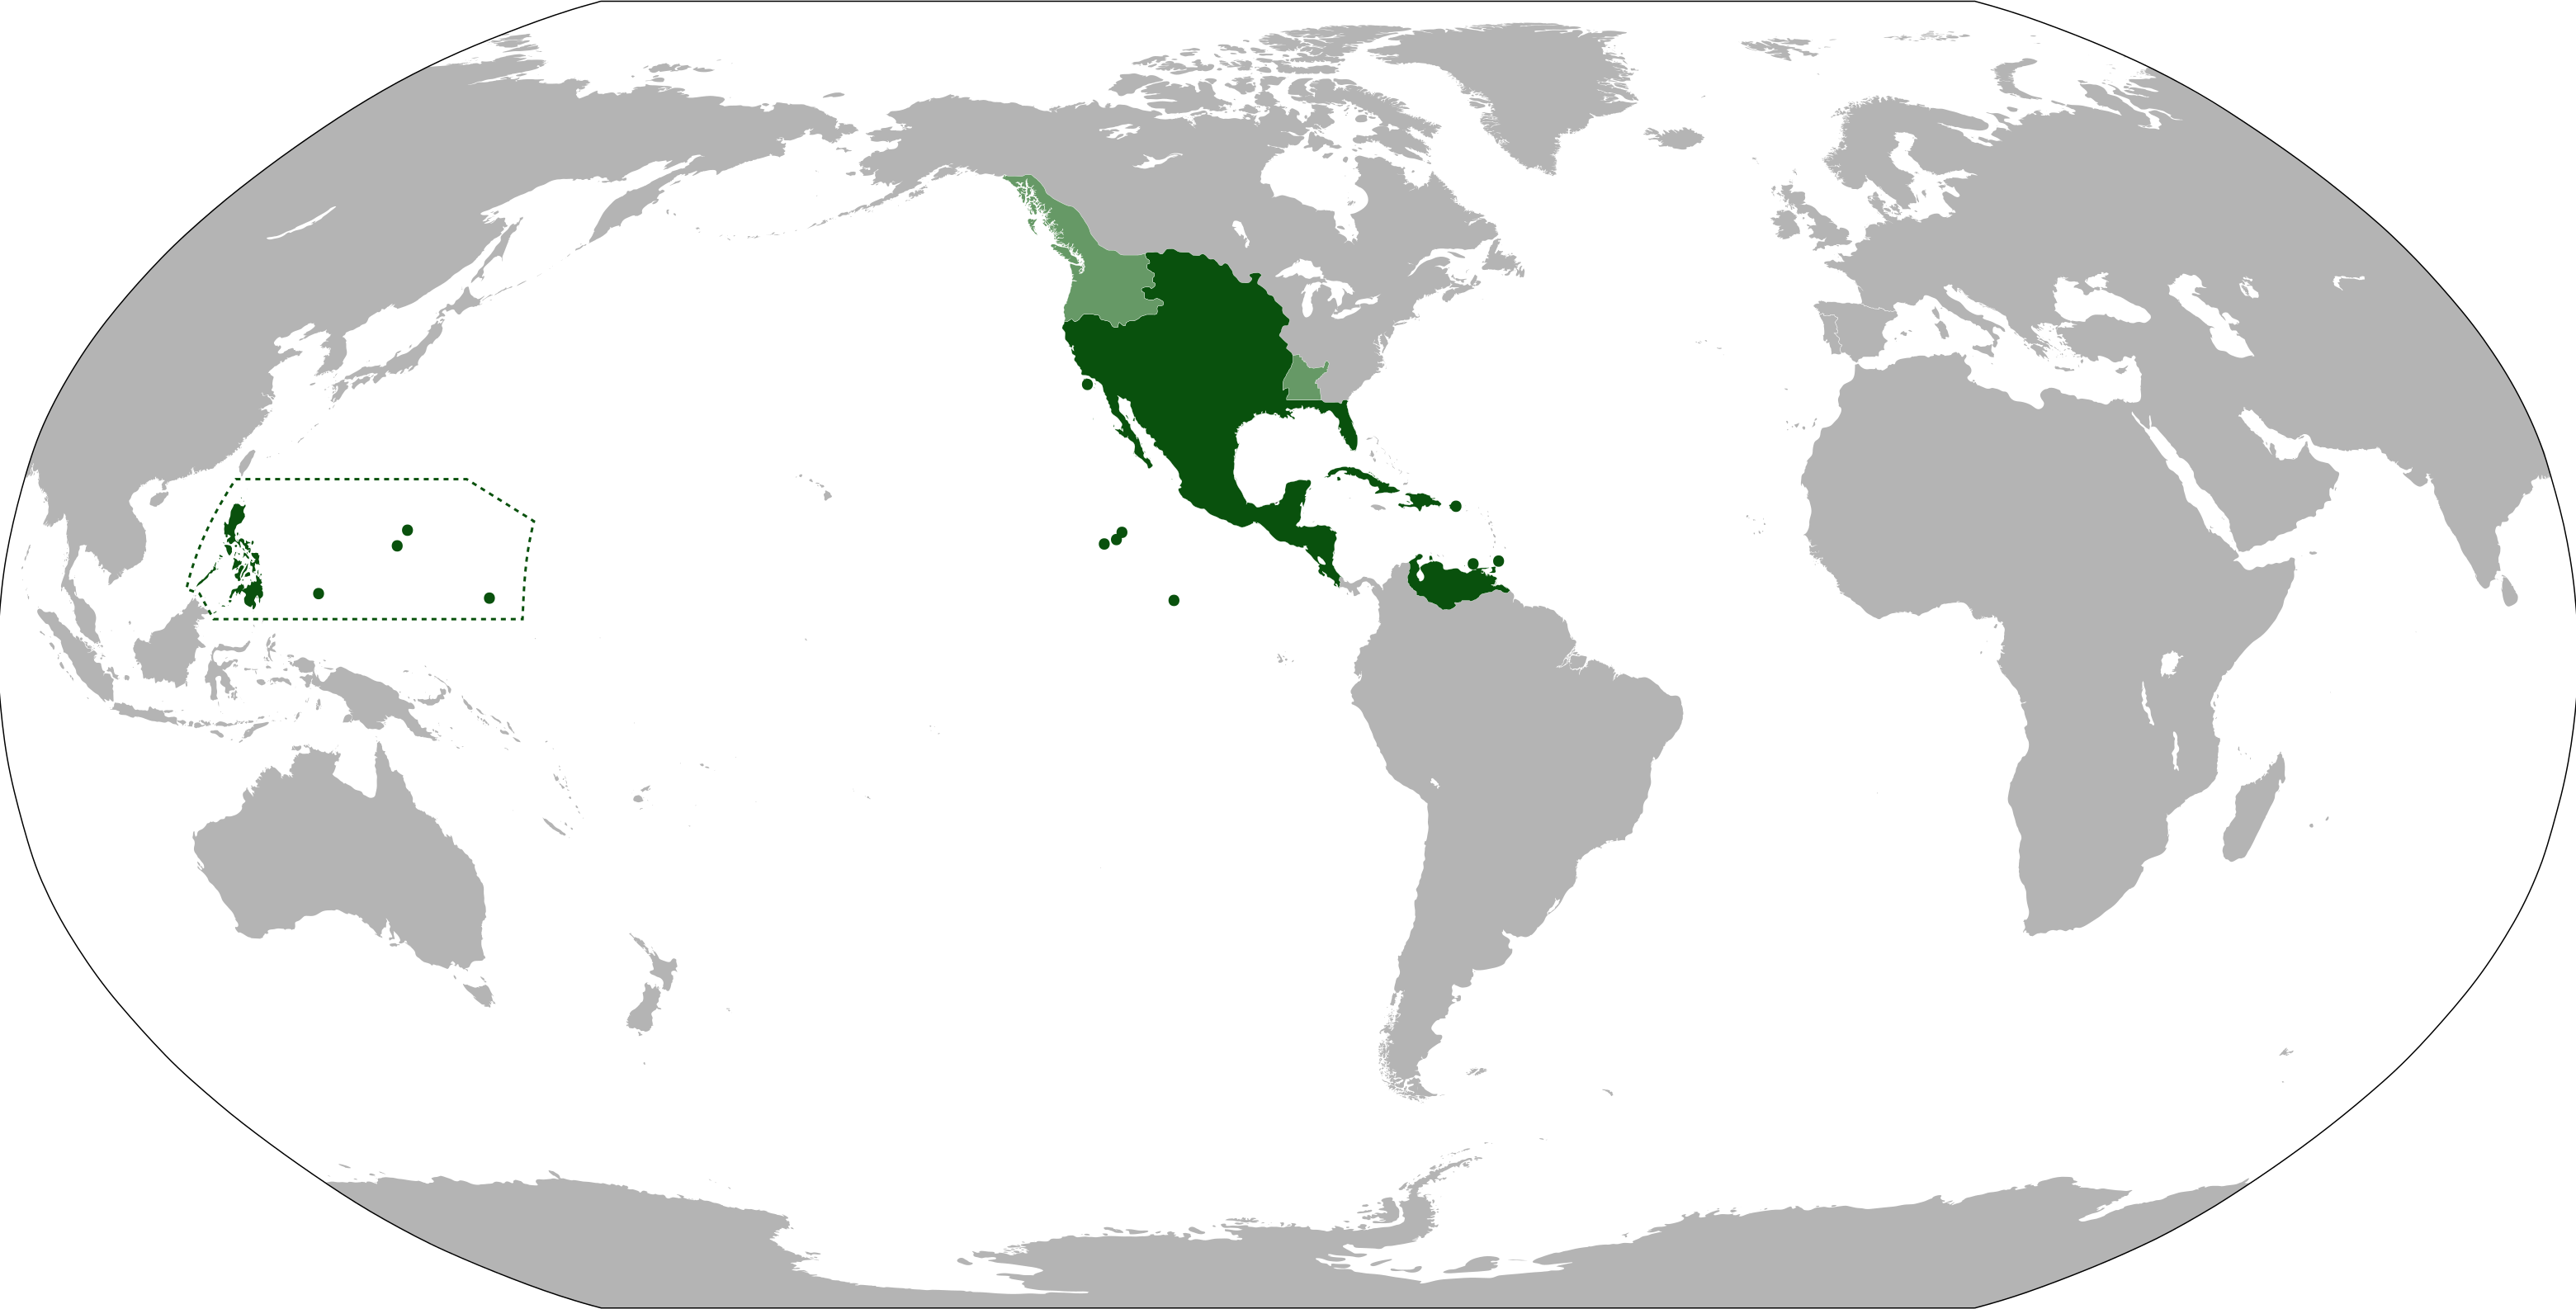
\includegraphics[width=10cm]{figures/vice.png}
\caption{The largest extent of the (northern) Spanish colonies in America, up to 1803.}
\end{figure}
\end{frame}

\begin{frame}{Nomenclature: geographic and political}
\footnotesize
The four major Spanish \textit{virreinatos}: a local, political, social, and administrative institution, created by the Spanish monarchy in the sixteenth century, for ruling its overseas territories.
\begin{itemize}
\footnotesize
\item \textbf{Virreinato de Nueva Espa\~{n}a}, former Aztec empire
\begin{enumerate}
\footnotesize
\item Capital: Ciudad de M\'{e}xico, Tenotchitlan, modern Mexico City
\end{enumerate}
\item \textbf{Virreinato del Per\'{u}}, former Incan empire
\begin{enumerate}
\footnotesize
\item Captial: Lima, Per\'{u}.  The original capital of the Incans was Cusco.  \textit{Note: Incan empire was the largest in the world at the time.}
\end{enumerate}
\item \textbf{Virreinato de Nueva Granada}, modern day Venezuela, Columbia, Panama, Ecuador
\begin{enumerate}
\footnotesize
\item Capital: Santa Fe de Bogot\'{a}, modern Bogot\'{a}, Colombia
\item Caracas and Quito are also within this province
\end{enumerate}
\item \textbf{Virreinato del R\'{i}o De la Plata}
\begin{enumerate}
\footnotesize
\item Capital: Buenos Aires
\item Modern Argentina, Chile, Bolivia, Paraguay and Uruguay
\end{enumerate}
\end{itemize}
\end{frame}

\begin{frame}{Nomenclature: geographic and political}
\begin{figure}
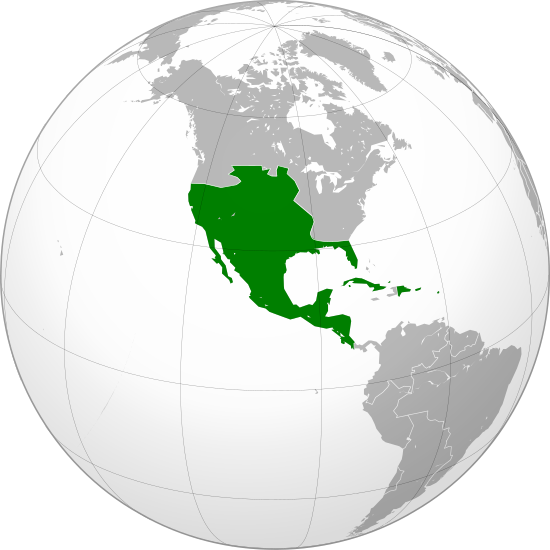
\includegraphics[width=6cm]{figures/vice_nuevaespana.png}
\caption{Virreinato de Nueva Espa\~{n}a}
\end{figure}
\end{frame}

\begin{frame}{Nomenclature: geographic and political}
\begin{figure}
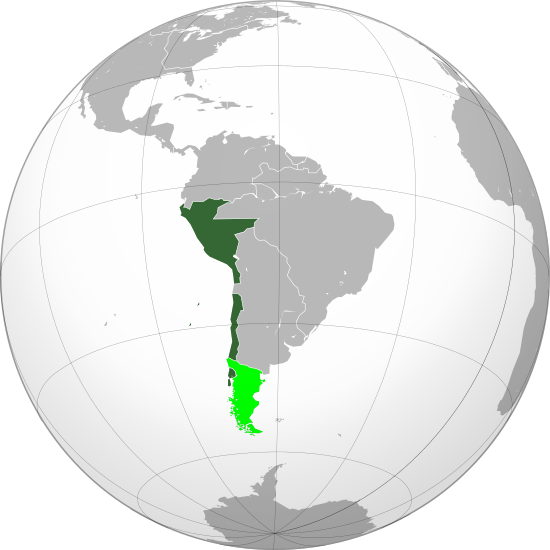
\includegraphics[width=6cm]{figures/vice_peru.png}
\caption{Virreinato del Per\'{u}}
\end{figure}
\end{frame}

\begin{frame}{Nomenclature: geographic and political}
\begin{figure}
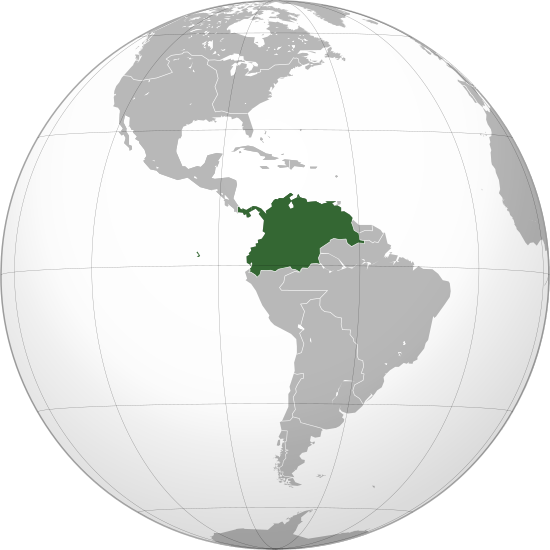
\includegraphics[width=6cm]{figures/vice_nuevagranada.png}
\caption{Virreinato de Nueva Granada}
\end{figure}
\end{frame}

\begin{frame}{Nomenclature: geographic and political}
\begin{figure}
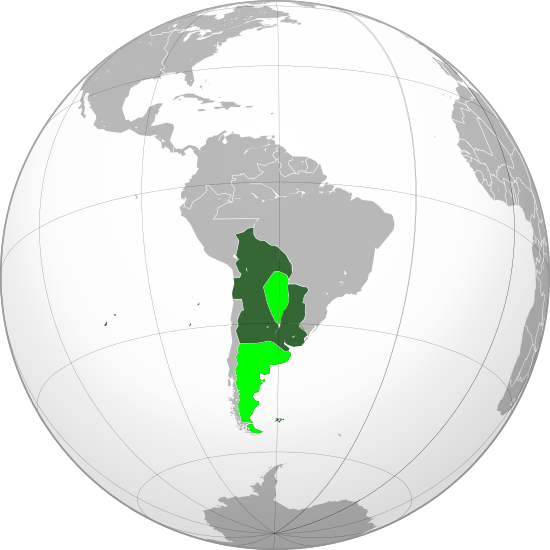
\includegraphics[width=6cm]{figures/vice_riodelaplata.png}
\caption{Virreinato del R\'{i}o De la Plata}
\end{figure}
\end{frame}

\begin{frame}{Nomenclature: Nahuatl and Espa\~{n}ol}
\small
\begin{columns}[T]
\begin{column}{0.65\textwidth}
Consider these 8 words, from English:
\begin{enumerate}
\item Chocolate (cocoa)
\item Coyote
\item Avocado
\item Tomato
\item Chili
\item Ocelot
\item Axolotl (some say: Texas salamander, cave salamander)
\item Chipotle
\end{enumerate}
\end{column}
\begin{column}{0.35\textwidth}
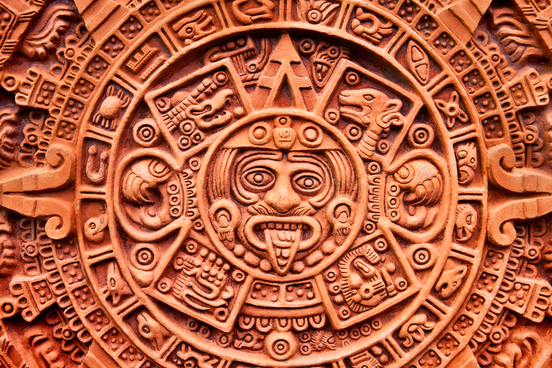
\includegraphics[width=0.9\textwidth]{figures/aztec.jpg}
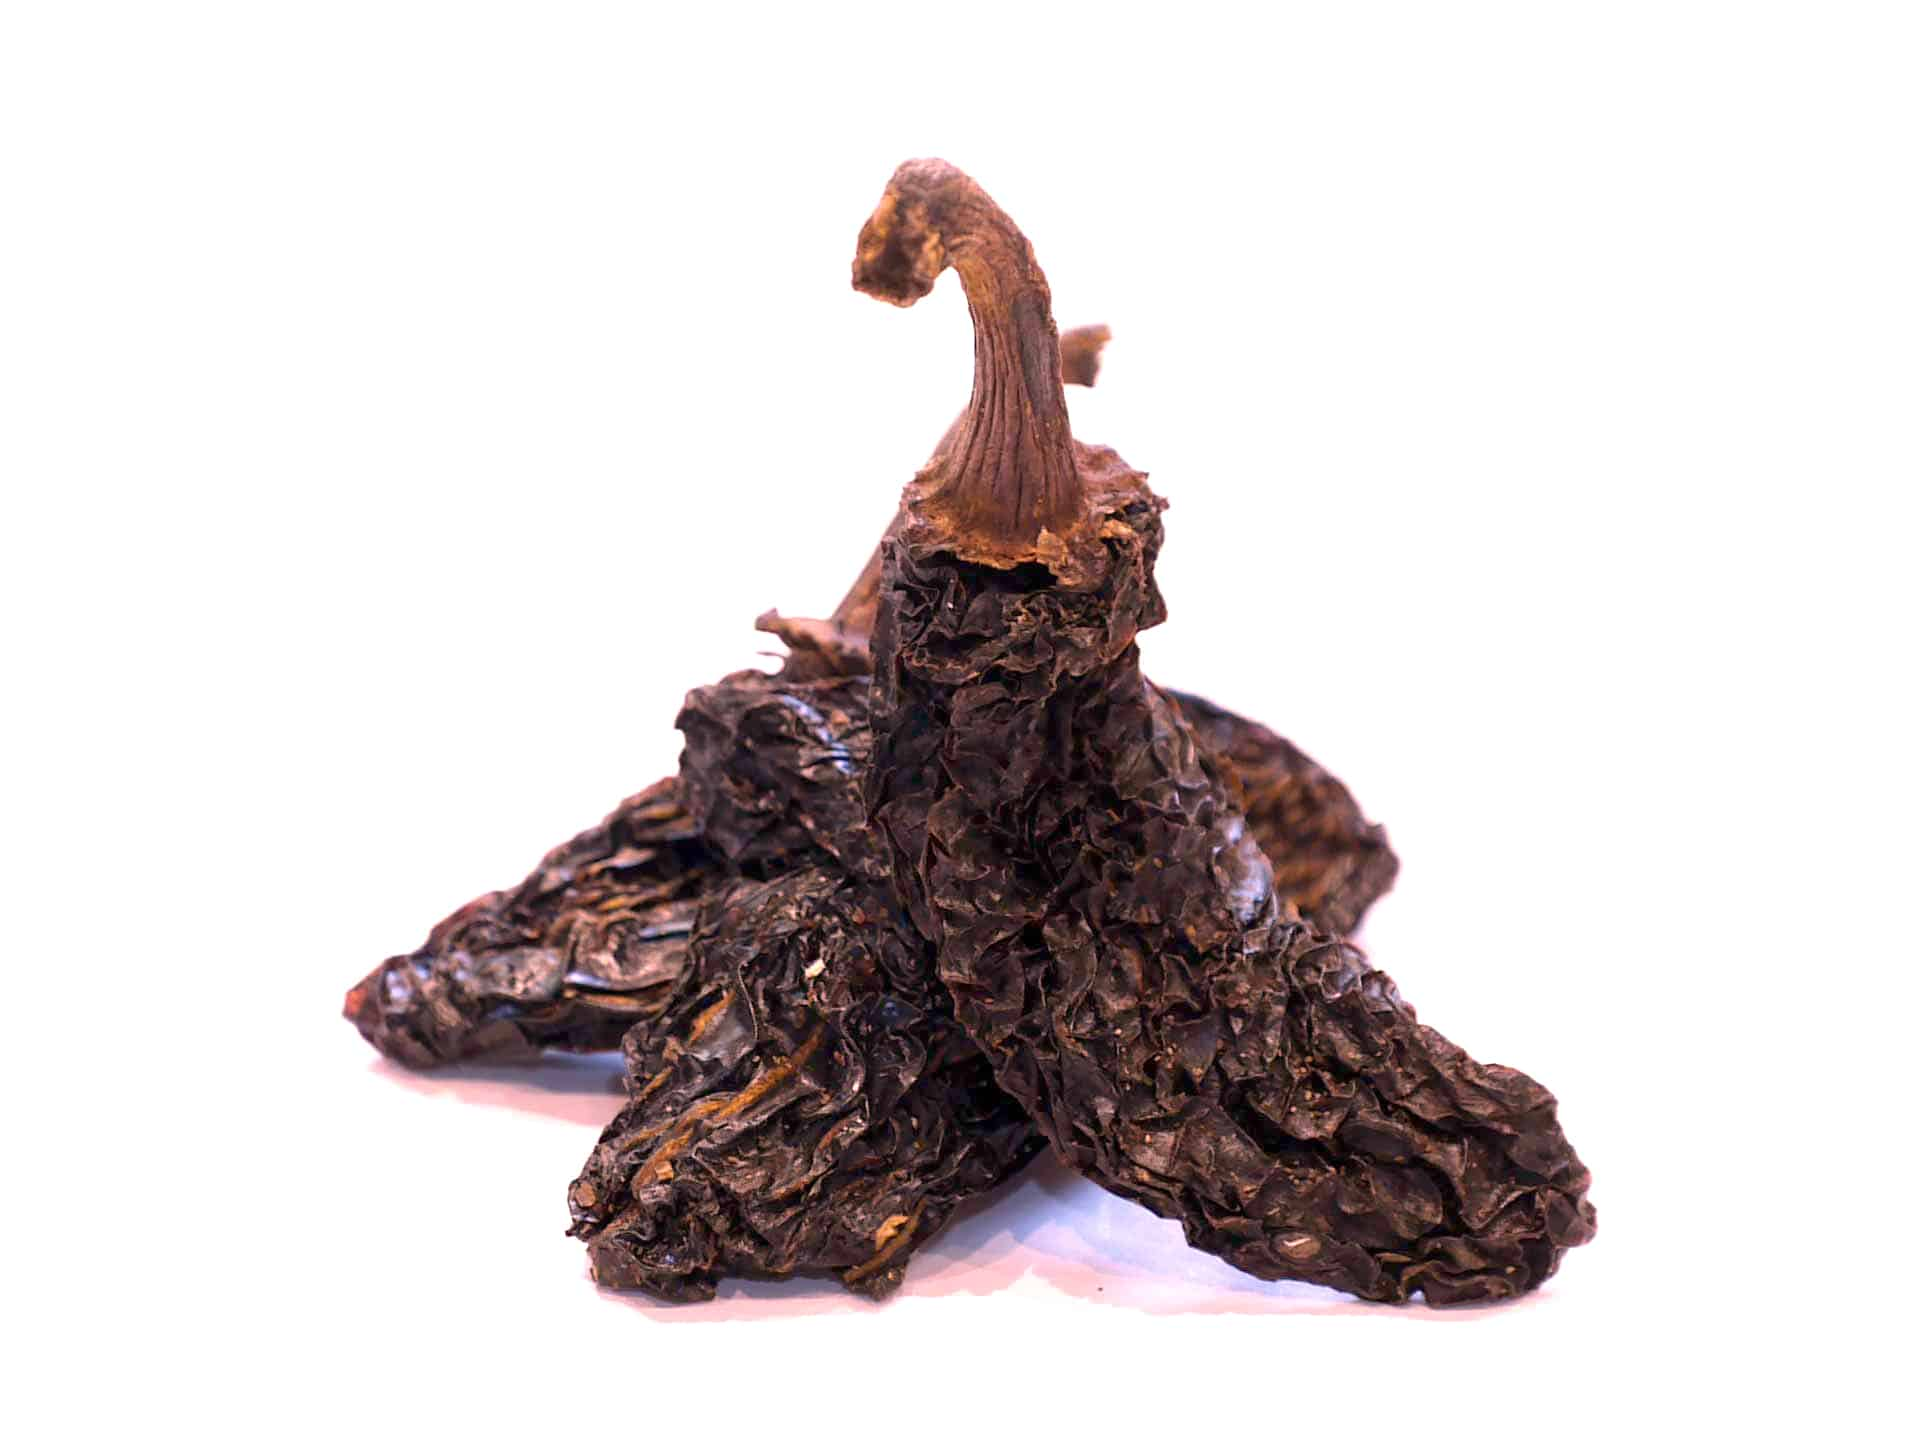
\includegraphics[width=0.9\textwidth]{figures/chipotle.jpg}

\includegraphics[width=0.9\textwidth]{figures/axolotl.jpeg}
\end{column}
\end{columns}

\end{frame}

\begin{frame}{Nomenclature: Nahuatl and Espa\~{n}ol}
\small
Trace the words through history:
\begin{enumerate}
\item Chocolate ... chocolate (Esp.) ... chocolatl
\item Cocoa ... cacao (Esp.) ... cacahuatl ... peanut, or cocoa bean
\item Coyote ... coyote (Esp.) ... coyotl
\item Avocado ... aguacate (Esp.) ... ahuacatl\footnote{This is also the word for testicle.}
\item Tomato ... tomate (Esp.) ... tomatl
\item Chili ... chile (Esp.) ... chilli
\item Ocelot ... ocelot (Fr.) ... ocelotl
\item Axolotl (a salamander) ... axolotl
\item Chipotle ... chipotle (Esp.) ... chilli + poctli = chilpoctli.  Smoked jalape\~{n}o, chile from Xalapa.
\end{enumerate}
\vspace{0.5cm}
\end{frame}

\begin{frame}{Nomenclature: Nahuatl and Espa\~{n}ol}
\small
More Nahuatl vocabulary\footnote{The Spanish x makes a sound much like the English ``h,'' as in \textit{M\'{e}xico} or \textit{Oaxaca}, but in Nahuatl it's closer to the English ``sh.''  The ``tl'' in Nahuatl does not exist in English or the Romance languages, so it takes some practice.}:
\begin{enumerate}
\item \textbf{Nahua}: main ethnic group indigenous to Mexico.  The Aztecs were of Nahua ethnicity.  Around 500 BC, settled in the basin in central Mexico.
\item \textbf{Nahautl}: a language group of the Nahua
\item \textbf{altepetl}: a Nahua city-state within which most individuals were of the same tribe and ethnicity.  Sub-unit: \textbf{calpolli.}
\item \textbf{amoxtli}: a codex or book written in Nahuatl
\item \textbf{tlacuiloll}: a painting or stelae
\item \textbf{tlacuilo}: one who paints or records, a notary or scribe
\end{enumerate}
\vspace{0.5cm}
\end{frame}

\begin{frame}{Nomenclature: Nahuatl and Espa\~{n}ol}
\small
\begin{enumerate}
\small
\item \textbf{Nahuatl list of animals}: \footnotesize \url{http://www.native-languages.org/nahuatl_animals.htm}.
\small
\item Fun story: \textit{la historia del tecolote y mi suegra.  B\'{u}ho o tecolote?}
\item \textbf{Quetzal}: a tropical bird that carries the same name today
\item \textbf{Coatl}: a snake
\item \textbf{Quetzalcoatl}: Aztec deity (feathered serpent), related to wind, Venus, the Sun, knowledge, and learning
\item \textbf{Quetzalcoatlus}: a dinosaur \\ \footnotesize \url{https://youtu.be/zWGnlAQsRaE?si=co-Uqi1ZBZzIt-xo}
\end{enumerate}
\end{frame}

\begin{frame}{Nomenclature: Nahuatl and Espa\~{n}ol}
Try: condor (from Quechua, originally), \textbf{cozcacuauhtli}, ... griffin?
\begin{figure}
\centering
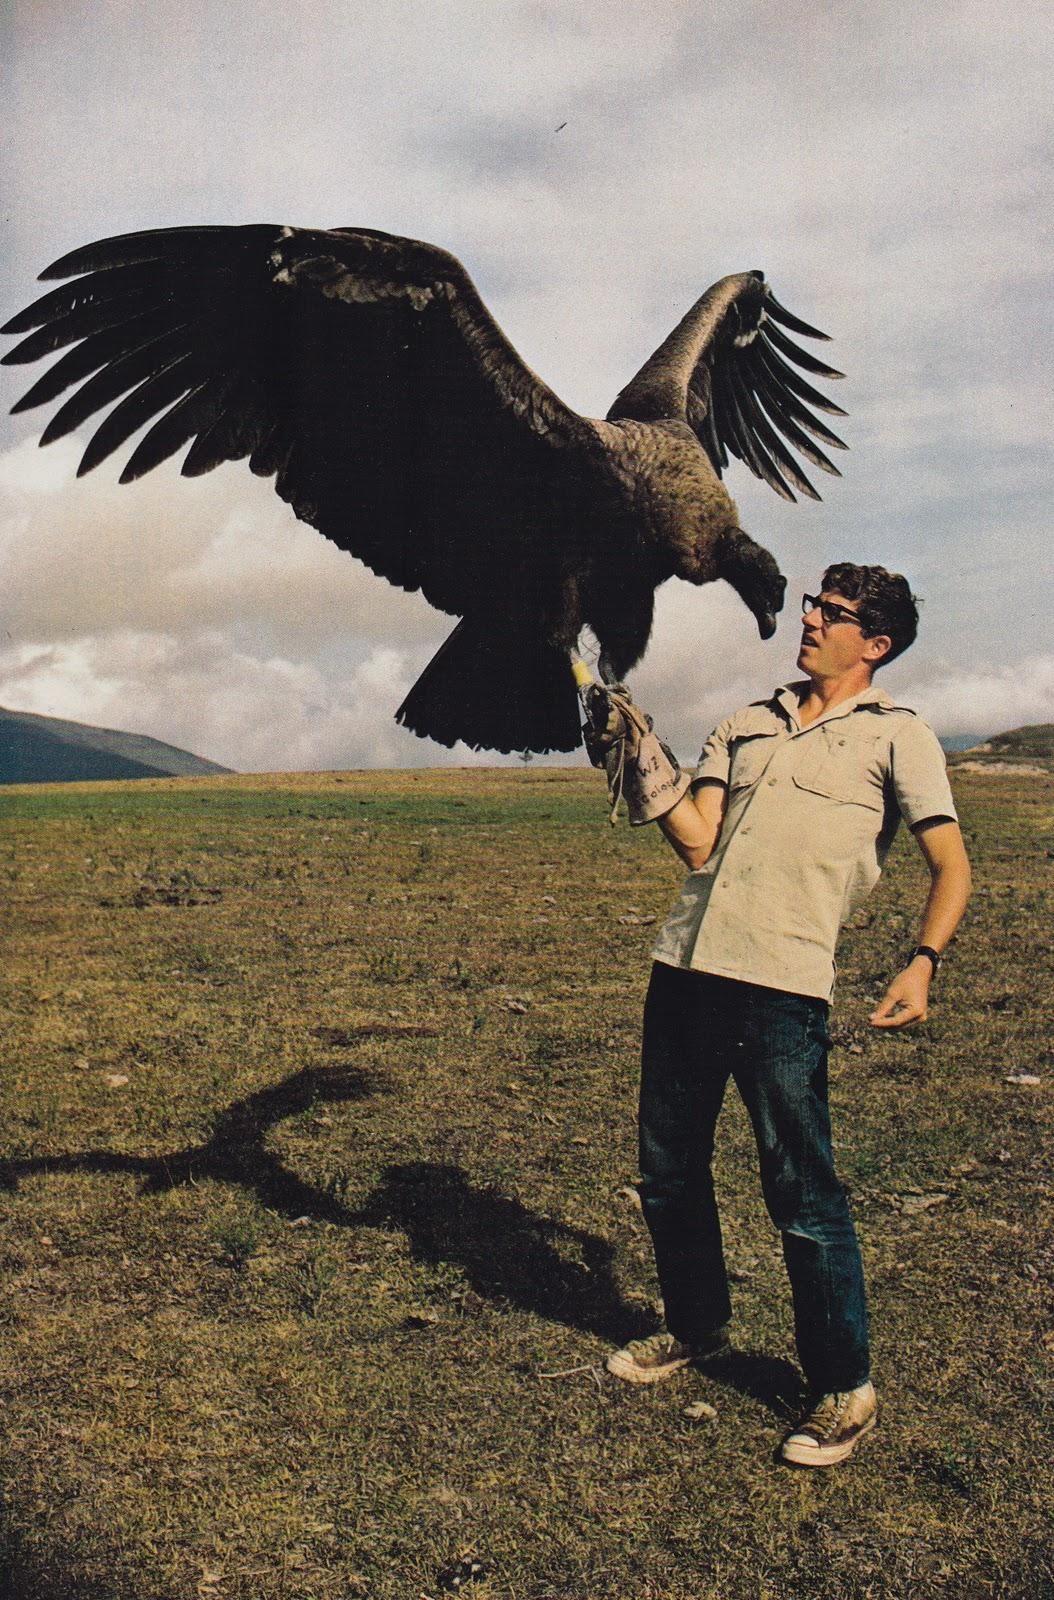
\includegraphics[width=3cm]{figures/condor.jpg}
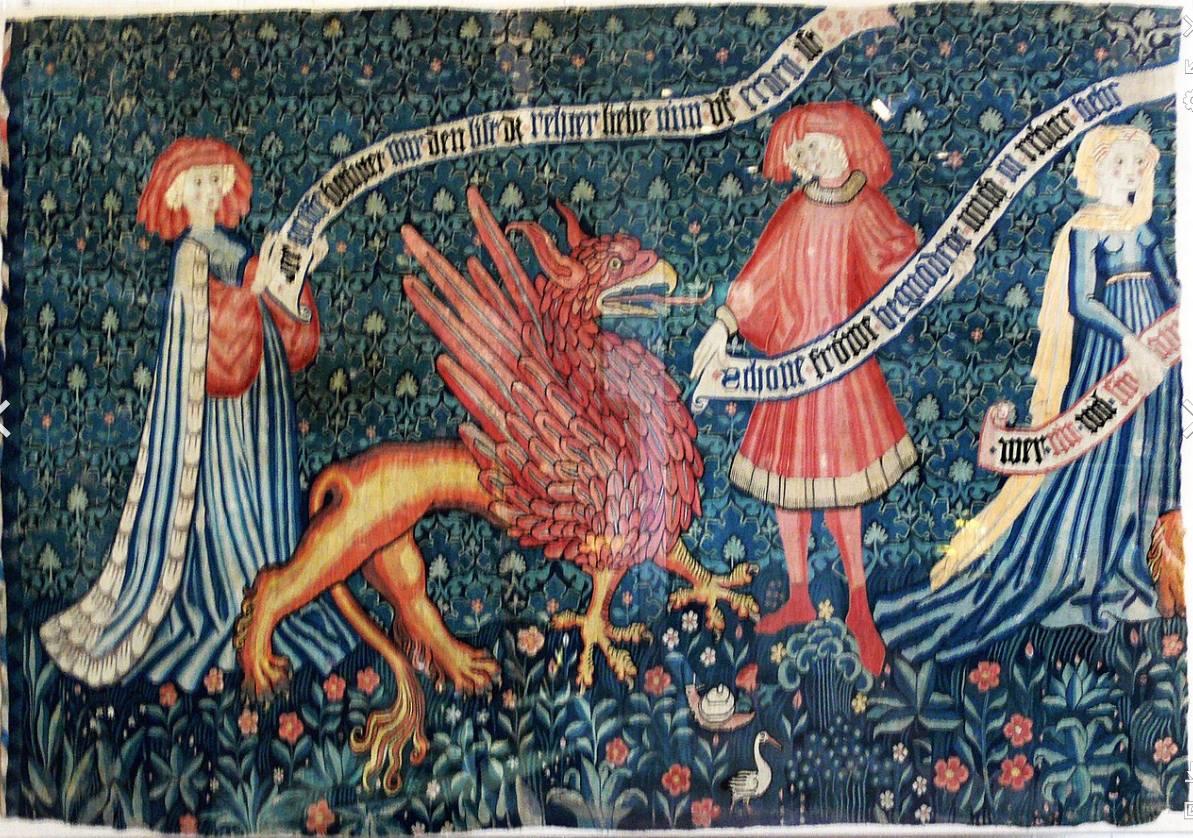
\includegraphics[width=6cm]{figures/griff.png}
\caption{(Left) A California condor to scale with a man.  (Right) Colonials compared this creature to a classical griffin.}
\end{figure}
\end{frame}

\begin{frame}{Nomenclature: Nahuatl and Espa\~{n}ol}
\small
Some medical terminology (balm, balsam)
\begin{enumerate}
\item \textbf{Xilo, xiloxochitl}: balsam, balsam tree.  A general term for residue extracted from tree matter that has medicinal properties.  The word balsam comes from The Balm of Gilead, in the Hebrew Bible (Genesis) for a region currently in Jordan.  Why did the Spanish colonials refer to \textit{xilo} as balsam?
\item \textbf{tzipipatli}: an herb native to Nueva Espa\~{n}a used to treat diarrhea.  Compare to how the Europeans treated diarrhea.
\item \textbf{atolli}, \textbf{atole} (Esp.) A thick, starchy drink made with water, maize (masa), milk/condensed milk, with chocolate and cinnamon: \alert{champurrado}.  Atole is sometimes used as a way to ease digestion, or clear the intestines
\end{enumerate}
\end{frame}

\section{Conclusion}

\begin{frame}{Unit 0 Summary}
\footnotesize
\textbf{The Scientific Attitude, Nomenclature, Mesoamerican Science}
\begin{enumerate}
\item The Demarcation Problem: the line between science and non-science
\item Nomenclature: philosophical, ecclesiastical, geographical, and political
\item \textit{Reading and discussion}
\begin{itemize}
\footnotesize
\item \alert{The Introduction and Chapter 1 of \textit{The Scientific Attitude}}
\begin{enumerate}
\item Examples of good science in 19th century medicine
\item Examples of denialism, pseudo-science, and fraud
\end{enumerate}
\item \alert{Introduction and Chapter 1 of \textit{Science in Latin America}}
\begin{enumerate}
\item Examples of botany, zoology, and medicine of indigenous 18th-century Mexican people
\item Comparisons to colonial knowledge and medieval medicine
\item Examples of knowledge transmission: Europe to Latin America, and Latin America to Europe
\end{enumerate}
\end{itemize}
\end{enumerate}
\end{frame}

\end{document}
